\lettrine{L}{a} rete è stata implementata come una rete  \textbf{\textit{p2p decentralizzata ibrida e non strutturata}}, composta da:
\begin{itemize}
\item[•] un \textbf{server} centrale, il cui unico compito è quello di tenere una lista dei peer che si sono connessi alla rete chiedendo ad esso l'autorizzazione.
\item[•] un numero dinamico di \textbf{peer}, che costituiscono la overlay network e mantengono la blockchain. 
\item[•] un numero indefinito di \textbf{wallet} che costituiscono i client dei peer e che permettono all'utente di effettuare varie transazioni di \vitcoin.
\end{itemize}

\begin{SCfigure}
  \centering
  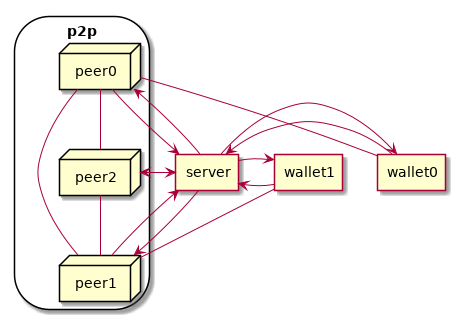
\includegraphics[scale=0.45]{arch.png}    
  \caption[architettura della rete]{\textbf{architettura della rete}: rappresentazione grafica della rete descritta sopra.\\ Le connessioni sono rappresentate dalle linee semplici, mentre le frecce rappresentano lo scambio di informazioni}
\end{SCfigure}

\section{Server}
Il server si occupa solo ed esclusivamente di dell'indirizzamento delle connessioni. Tale compito si divide sostanzialmente in 3 sottocompiti:
\begin{itemize}
\item indicare ad i nuovi peer, i peer a cui connettersi.
\item indicare ad i wallet, il peer a cui connettersi.
\item eliminare i peer che si autoterminano, dalla lista che rappresenta la rete.
\end{itemize}
 
\section{Peer}
Un peer in quanto tale, si comporta sia da \textit{client}(verso altri peer e il server) che da \textit{server} (verso altri peer e verso i wallet ad esso collegato).\\ Esso di  occupa sostanzialmente di effettuare 3 macro compiti:
\begin{itemize}
\item[•] \textit{mantenere la rete p2p}, stabilendo e gestendo le connessioni con gli altri peer.
\item[•] \textit{gestire la blockchain}, aggiornandola con i blocchi provenienti dagli altri peer e diffondendo i blocchi creati.
\item[•] \textit{soddisfare le rischieste di un wallet}, interagendo  con la blockchain leggendo o inserendo blocchi che riguardano il wallet stesso. 
\end{itemize}

\section{Wallet}
Il wallet consiste nel client messo a disposizione per gestire il proprio portafogli di \vitcoin. Esso interagendo con il peer assegnatogli dal server permette di:
\begin{itemize}
\item[•] \textit{"mining"} di nuovi \vitcoin. 
\item[•] effetuare una transazione verso un altro wallet.
\item[•] richiedere un refresh del bilancio del wallet.
\end{itemize}
